\subsection{Дисперсионное соотношение для гравитационно-капиллярных волн на воде. Фазовая и групповая скорости волн. Нормальная и аномальная дисперсия.}
Гравитационным волнам на воде присуще явление фазовой дисперсии, т.е. зависимости скорости распространения от длины волны.
Волна, как единое образование, не может распространяться продолжительное время, поэтому она начинает диспергировать, т.е. распадаться на пакет волн с разной длиной волны \cite{Носов-2019-13}.
Тем не менее, например, существует явление солитона\footnote{Солитон -- структурно устойчивая уединённая волна.}.
Его образование объясняется наличием балансирующей амплитудной дисперсии, т.е. зависимости скорости распространения от амплитуды волны (чем больше амплитуда волны, тем больше её скорость).

Фазовая дисперсия бывает двух видов \cite{Носов-2019-13}:
\begin{enumerate}
\item Нормальная дисперсия: чем больше длина волны, тем больше её скорость (быстрее бегут длинные волны). Характерна для гравитационных волн.
\item Аномальная дисперсия: чем меньше длина волны, тем больше её скорость (быстрее бегут короткие волны). Характерна для капиллярных волн.
\end{enumerate}

Фазовая и групповая скорости волн определяются из дисперсионного соотношения\footnote{Дисперсионное соотношение -- зависимость вида $\omega=\omega(k)$.}:
\begin{equation}
v_\text{ф}=\frac{\omega}{k}\quad v_\text{гр}=\frac{d\omega}{dk}
\end{equation}
где $\omega$ -- угловая частота волны, $k=\frac{2\pi}{\lambda}$ -- волновое число.
Их спектр изображён на рис. \ref{fig:v_spectrum}.

Дисперсионное соотношение для гравитационных волн \cite{Носов-2021}:
\begin{equation}
\omega^2=gk\th(kH)
\end{equation}
Дисперсионное соотношение для капиллярных волн \cite{Носов-2021}:
\begin{equation}
\omega^2=\frac{\sigma}{\rho}k^3\th(kH)
\end{equation}
где $\sigma$ -- коэффициент поверхностного натяжения жидкости.

Дисперсионное соотношение для гравитационно-капиллярных волн \cite{Носов-2021}:
\begin{equation}
\omega^2=\left(gk+\frac{\sigma}{\rho}k^3\right)\th(kH)
\end{equation}

\begin{figure}[!ht]
\centering
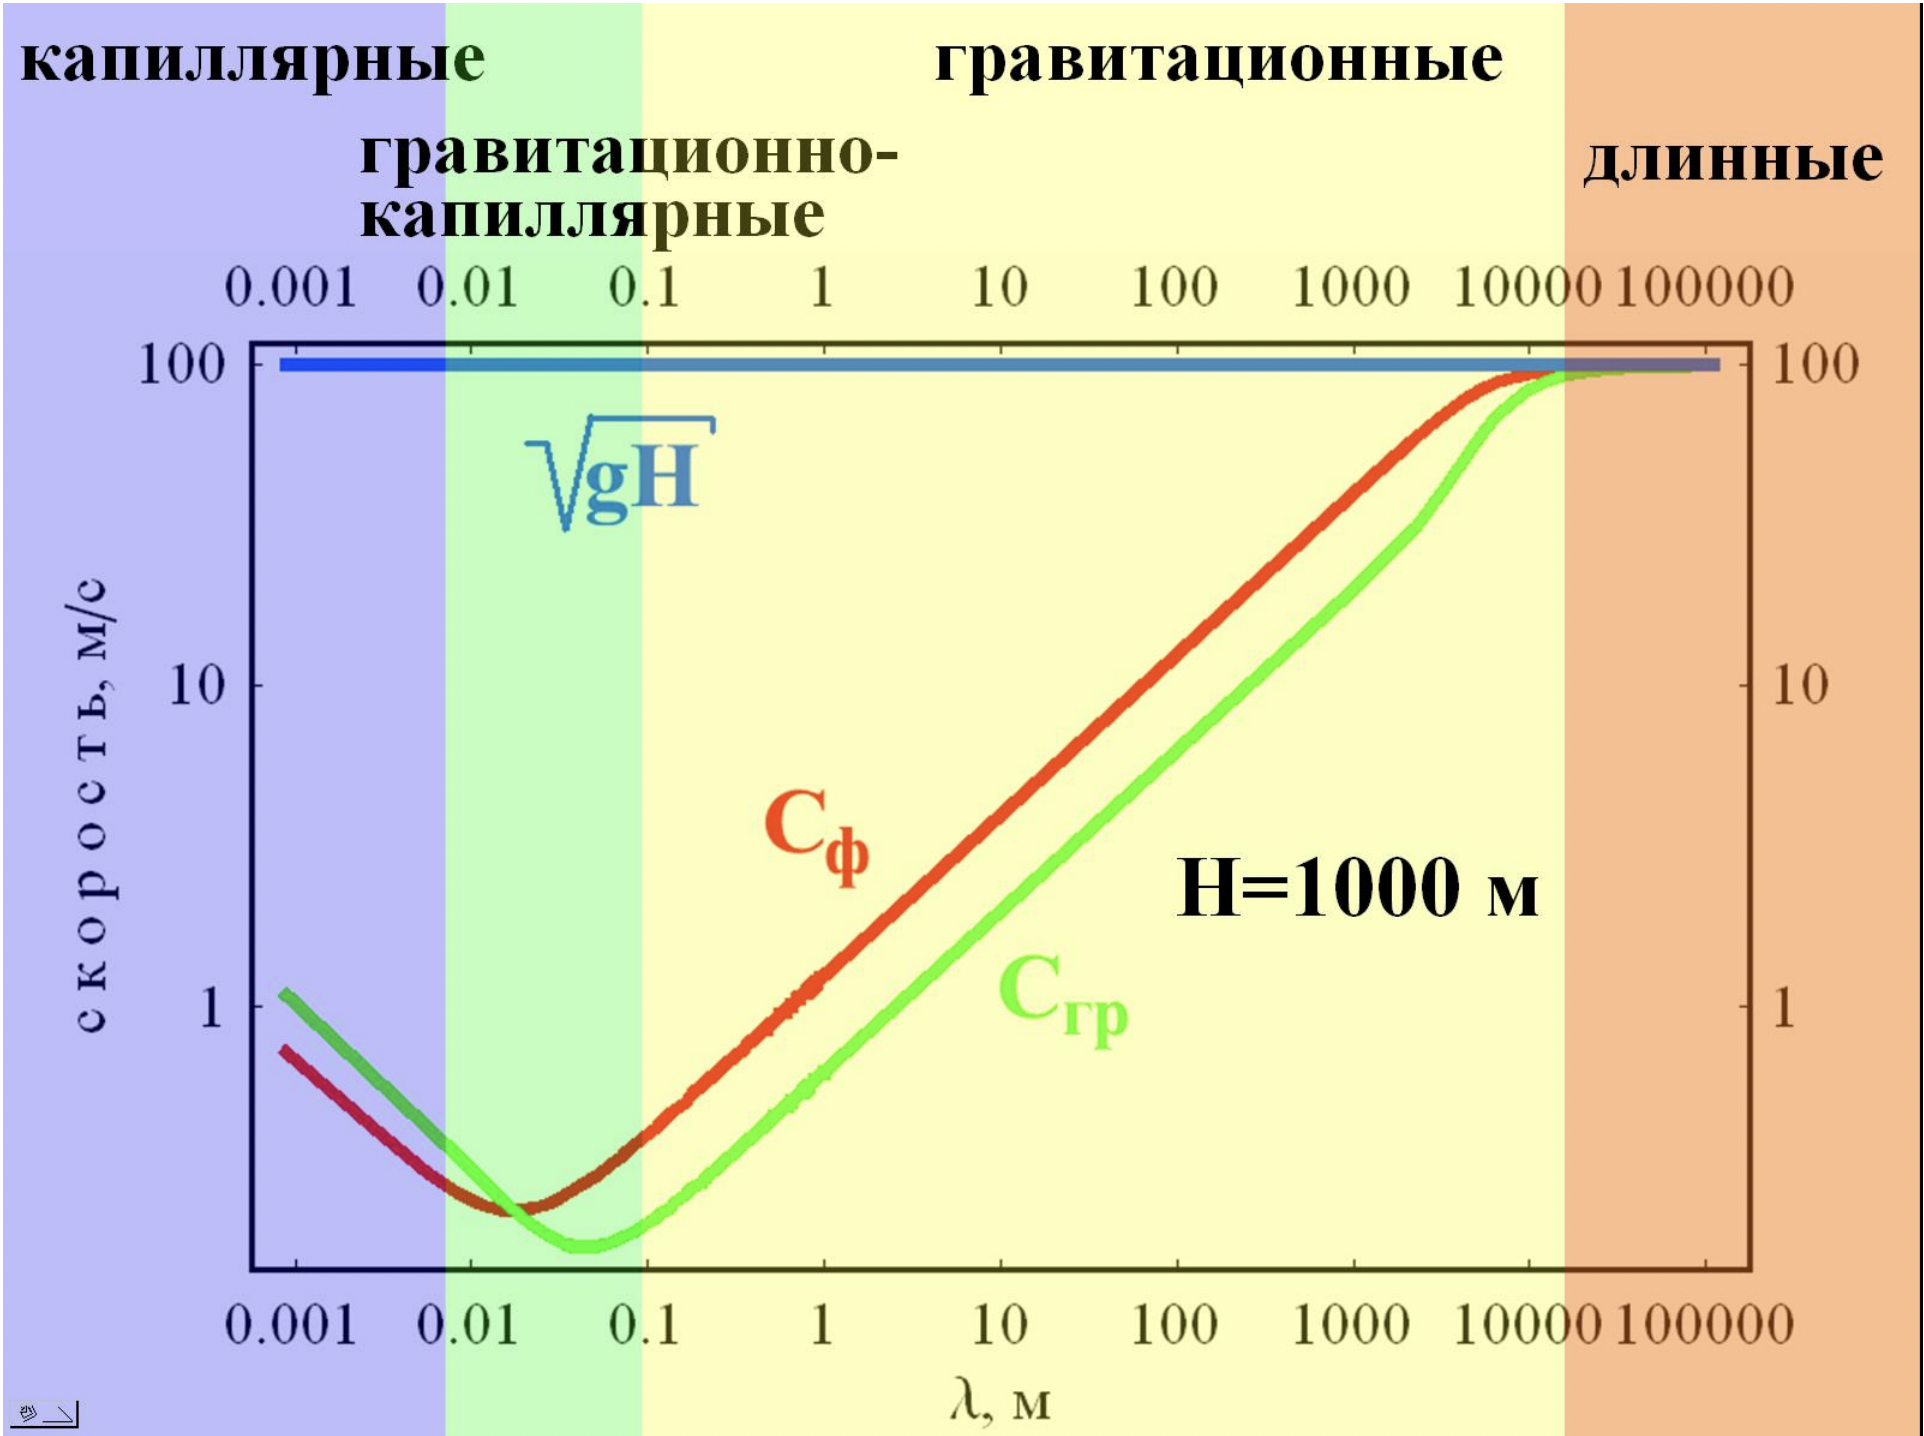
\includegraphics[width=0.5\textwidth]{images/v_spectrum.png}
\caption{Спектр скоростей волн \cite{Носов-2019-13}.}\label{fig:v_spectrum}
\end{figure}
